%!TEX root = ../3dbook.tex

\setchapterpreamble[u]{\margintoc}

\graphicspath{{voxels/}}
% \renewcommand*{\thelesson}{2.1}

\chapter{Voxels and voxelisation}%
\label{chap:voxels}

Voxel models, which are the 3D equivalent of 2D rasters, are a common way to store 3D models of the built environment using a regular 3D grid (Figure~\ref{fig:model}).
Much like rasters in 2D, they have inherent limits in precision based on the grid size that is used and can easily grow to very large sizes in terms of memory, especially with a small grid size and when compression is not used.

At the same time, voxel models are easy to use and understand, and algorithms to process them are typically much simpler than those using other representations, which also makes them more reliable, robust and easy to parallelise.
They also work well for both objects (by storing which objects are present in each voxel) and fields (by storing the field value in each voxel).
These characteristics make voxels an important and widely used representation to process 3D information in general.

\begin{figure}[htbp]
\centering
\begin{subfigure}[b]{\linewidth}
\includegraphics[width=\linewidth]{figs/model-pre}
\caption{}%
\label{subfig:model-pre}
\end{subfigure}
\\
\begin{subfigure}[b]{\linewidth}
\includegraphics[width=\linewidth]{figs/model-post}
\caption{}%
\label{subfig:model-post}
\end{subfigure}
\caption[A mesh model and a corresponding voxel model]{(a) A mesh model of a house with surrounding terrain and trees and (b) a corresponding voxel model with the same elements.}%
\label{fig:model}
\end{figure}

\section{Exhaustive enumeration models}

Voxels might appear to be quite a unique data model in terms of 3D representations, but they are actually only the most used among a type of related representations, which are together usually referred to as \emph{exhaustive enumeration}\marginnote{exhaustive enumeration}\index{exhaustive enumeration}.
The specifics of these data models differ, but in general they represent objects by:

\begin{enumerate}

\item \textbf{defining the shape of a domain}\marginnote{voxel domain}\index{voxel domain} in which the objects to be represented fit, or alternatively in which the region of interest of a field fits, \eg\ a bounding box defined by their minimum and maximum coordinates along each axis;

\item \textbf{dividing the domain} using a structure of many \emph{cells}\marginnote{voxel cells}\index{voxel cells}, usually following a regular or semi-regular pattern that can be defined programmatically (as opposed to explicitly representing the shape of each individual cell), \eg\ a grid defined by the number of cells along each axis;

\item \textbf{specifying a well-defined order} passing once through each cell of the subdivision, usually also programmatically (as opposed to explicitly numbering each cell), \eg\ the order and direction of iteration of the axes in a grid;

\item \textbf{labelling each cell} with values that indicate the object(s) that are in it, or in the case of fields, the values of variable(s) at that location.
The values can then be \emph{encoded linearly} using the order defined in the previous step.

\end{enumerate}

We can thus say that what is represented in an exhaustive enumeration is usually composed of four elements: (i) a set of rules defining the shape of a domain, (ii) a set of rules on how to divide the domain into cells, (iii) a set of rules that define an order of the cells, and (iv) an encoded linear representation that represents objects or values for all cells.
However, out of these four elements, the first three are sets of rules that are generally very simple, and thus they are stored encoded in a minimal way or not at all (\ie\ only implied by the context).
For instance, the rules might be part of the specification of a particular data format.

Based on these standard characteristics, we can see that exhaustive enumeration representations use space differently from other data models.
In most geometric representations, much (or most) of the space and complexity of a data structure is devoted to creating a custom structure that individually describes the shape of the objects being represented.
By contrast, in exhaustive enumeration, objects' shapes are instead approximated using simple rules on a predefined structure, and the vast majority of the space is thus devoted to specifying which objects are present in which cells (or the values of a field in each cell).

That being said, the statements described above---which in the steps correspond to the actions that are done for a standard regular 3D grid with voxels---can all differ substantially.
By analysing different possibilities at each step, it is easy to see how the approach can be adapted and extended to form other types of representations.
For instance, consider the following example, which is arbitrarily chosen to be completely different from a typical voxel grid.

We can start by describing a space using an alternative method, \eg\ a b-rep representation of a domain with an arbitrarily complex shape.
Cells could then be specified using a \emph{constrained Delaunay tetrahedralisation} of the domain (using predefined rules for the addition of Steiner points).
The order of the cells could be specified based on the lexicographical order of the vertices of each tetrahedron.
Finally, the values of each tetrahedral cell are then encoded linearly as in a grid.

While the previous example is perfectly possible, it is worth noting that exhaustive enumeration schemes are well-liked largely because of their simplicity, which means that simpler representations are usually preferred.
Using a complex representation where the geometry is not trivial to compute on the fly (\eg\ a CDT) thus defeats many of the advantages of the exhaustive enumeration approach.

Most examples that are found in practice are thus relatively minor variations of voxel grids.
For instance, cells can have varying sizes according to their place in the grid (\eg\ when more details are desired in a particular region), the domains of grids can be stretched in some directions (such that the domain is oblique), or the cells can be of different shapes (\eg\ octahedra).

Among the variations of voxel grids, \textbf{sparse voxel models}\marginnote{sparse voxel model}\index{sparse voxel model} are used widely in practice to describe objects (\ie\ not fields) and are thus worth describing in more detail here.
These representations opt to encode only the voxels containing something (rather than all voxels in the domain).
In order to do so, they usually specify simple objects consisting of: (i) a voxel position, \eg\ using integer coordinates for its position along each axis, and (ii) the voxel's variables.
While this is undoubtedly more space-intensive per voxel than the standard encode-all approach, it works well for 3D models consist of largely empty space, which occurs frequently in 3D city models and where the objects we want to represent do not fit neatly into a box-shaped domain.

It is also worth pointing out that most variations of voxel models can be processed with basically the same methods as standard voxel grids.

\section{Hierarchical subdivision models}

In addition to exhaustive enumeration, there are also related data models where the structure is not entirely predefined, but it is instead defined hierarchically using space-partitioning trees.
The root of the tree thus refers to a predefined space that will be subdivided, which corresponds to the entirety of the domain that is represented in an exhaustive enumeration model.
Each node then specifies a subset of the space defined by its parent node, and nodes (usually but not necessarily at the leaf level) are then labelled to specify the object(s) or value(s) present in the space represented by it.

Since different branches of a tree do not need to have the same depth, hierarchical subdivision models can have different resolutions in different parts of the model, and can thus adapt to the shape of the objects being represented.
This allows them to act as more compact alternatives to exhaustive enumeration models in certain cases, usually where there are large objects that occupy many adjoining cells.
Note however that the tree structure of a hierarchical representation can occupy a significant amount of space.

Hierarchical subdivisions are also a good way to encode the sparse models described in the previous section, where large areas of empty space will be efficiently represented by leaf nodes that are generally close to the root of the tree.

The most common structures used by hierarchical subdivision models are:

\begin{description}

\item[octrees] subdivide space evenly along the \(x\), \(y\) and \(z\) axes into eight equal-size \emph{octants}.
They are analogous to quadtrees in 2D, which subdivide space evenly along the \(x\) and \(y\) axes into four equal-size quadrants.

\item[bintrees] are similar to octrees, but they subdivide space in halves along only one axis per node, then switching to a different axis for the next level of the tree, \eg\ \(x\), then \(y\), then \(z\), then \(x\) again, etc.

\item[\(k\)-d trees] are similar to bintrees, but they subdivide space using an arbitrary plane per node, which can be defined by a single coordinate included in the node.

\end{description}

\section{Conversions to and from voxels}

The process through which other data models are converted into voxels is often called \emph{voxelisation}\marginnote{voxelisation}\index{voxelisation}.
It is analogous to rasterisation in 2D.

\subsection{Voxelisation of fields}
 
The conversion from scattered points representing a field to a voxel grid is trivial: simply interpolate at regular locations in three dimensions% 
\index{interpolation}\marginnote{interpolation}
(which represent the centre of each voxel) and output the results in the appropriate format (grids can be stored in many ways). 
Figure~\ref{fig:r-interpolation} shows the process in two dimensions.
\begin{figure}
  \centering
  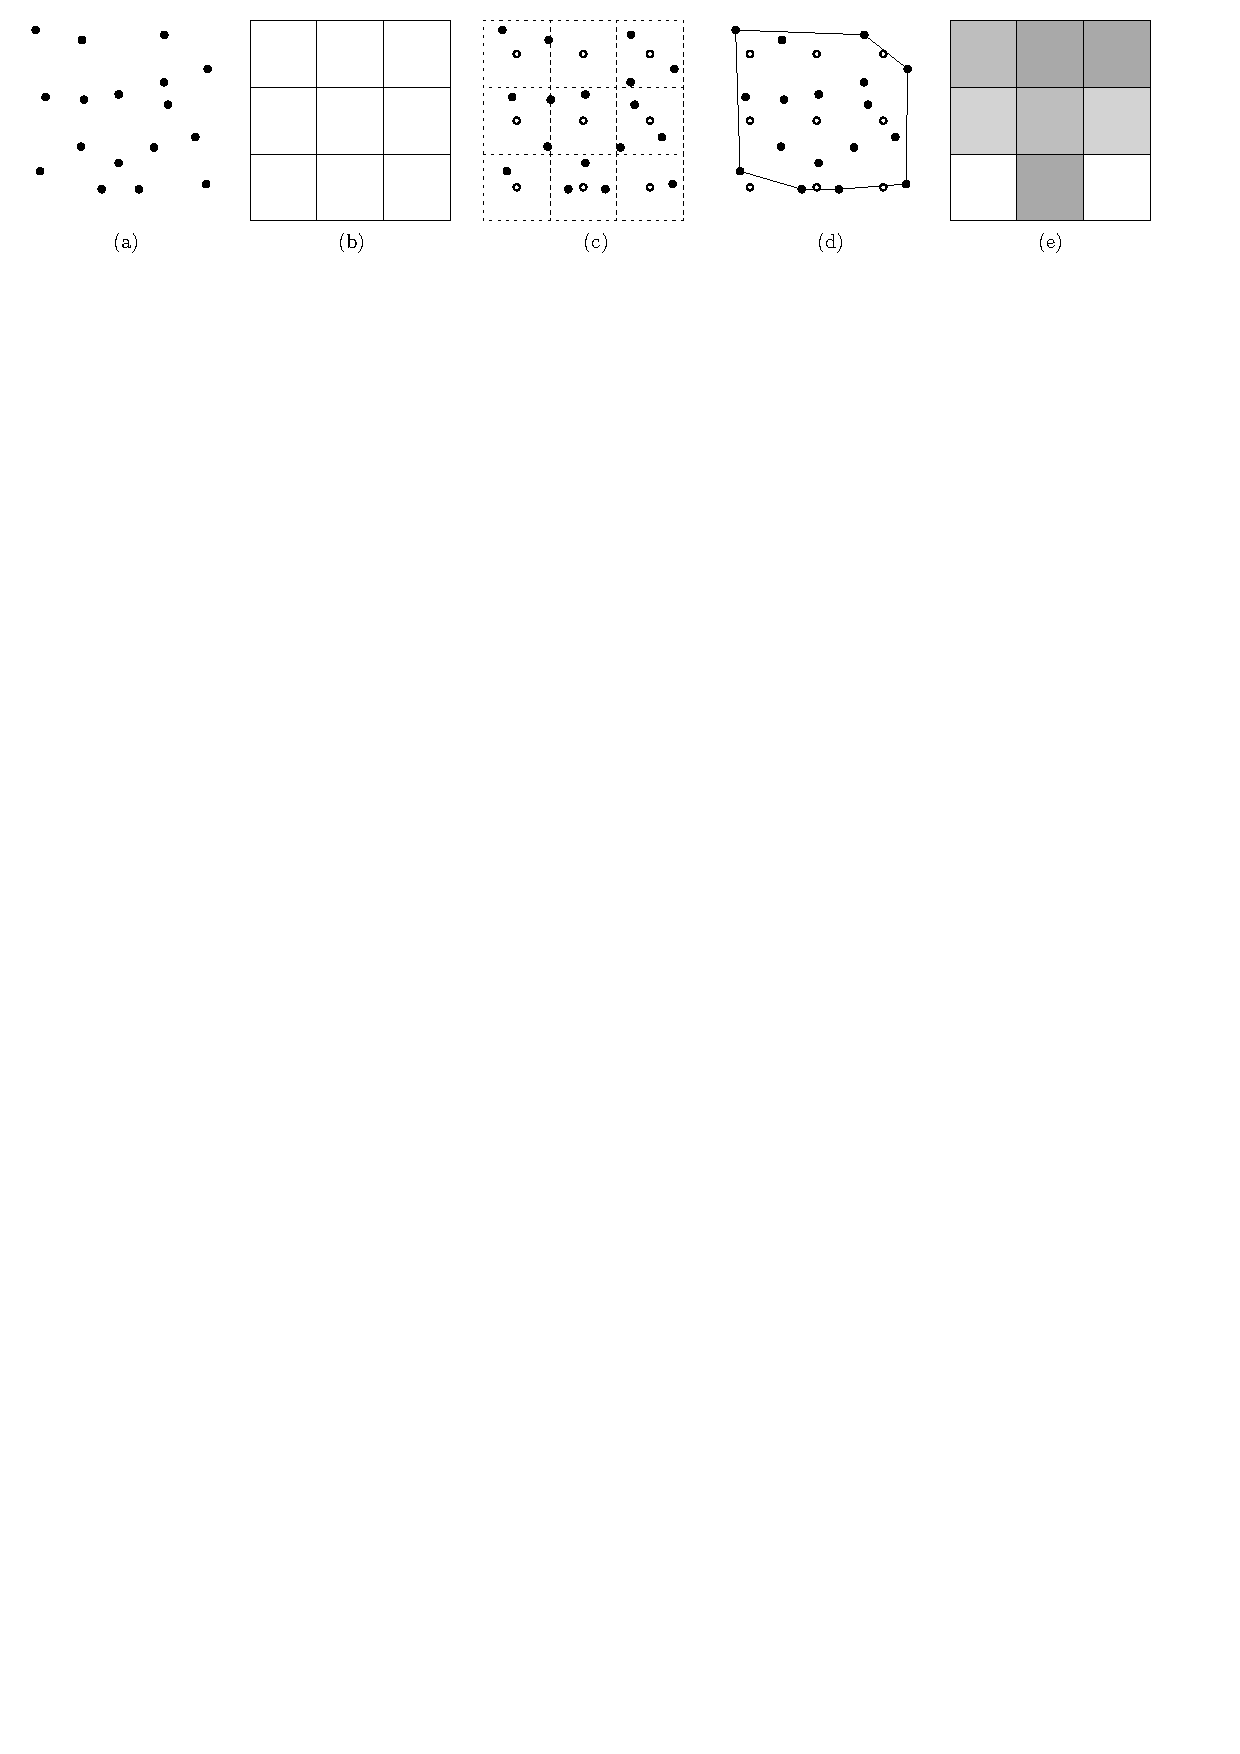
\includegraphics[width=\linewidth]{figs/r-interpolation}
  \caption[Interpolations of sample points into a raster]{\textbf{(a)} input sample points. \textbf{(b)} size/location of output grid. \textbf{(c)} 9 interpolations must be performed (at locations marked with $\circ$): at the middle of each cell. \textbf{(d)} the convex hull of the sample points show that 2 estimations are outside, thus no interpolation. \textbf{(e)} the resulting raster.}%
\label{fig:r-interpolation}
\end{figure}

\begin{kaobox}[frametitle=\faExternalLink\ To read or to watch.]
  The two chapters about spatial interpolation (Chapters~4 and 5) in the book \emph{Computational modelling of terrains}~\citep{terrain_book} cover related concepts and methods in 2D.
\end{kaobox}

All the two-dimensional interpolation methods (weighted-average and kriging) generalise in theory to three dimensions.
However, it is not obvious that they preserve their properties or are appropriate for geoscientific datasets.
We describe in the following how they can be, and their properties.

%%%
\paragraph{Nearest neighbour.} 
The method, based on the Voronoi diagram (VD),% 
\index{Voronoi diagram}\marginnote{Voronoi diagram}
generalises in a straightforward manner to 3D.
It suffices to build the VD and to identify inside which cell the interpolation point lies.
The VD can be bypassed if a three-dimensional $k$d-tree is used.


%%%
\paragraph{Inverse distance weighting (\textbf{IDW}).}
The generalisation of this method to three dimensions is straightforward: a searching \emph{sphere} with a given radius is used. 
The same problems with the one-dimensionality of the method (the value for the search radius) will be even worse because the search must be performed in one more dimension. 
The method has too many problems to be considered  has a viable solution for fields as found in geosciences: the interpolant is not guaranteed to be continuous, especially when the dataset has an anisotropic distribution, 
\marginnote{anisotropic distribution}
and the criterion has to be selected carefully by the user.
Note that the implementation problems are also similar to the ones encountered with the previous method, and an auxiliary data structure must be used to avoid testing all the points in a dataset.


%%%
\paragraph{Linear interpolation in tetrahedra.}
This is the generalisation of the popular linear interpolation in TINs where the tetrahedra of the Delaunay tetrahedralisation (DT) are used. 
The barycentric coordinates can be used to linearly interpolate inside a tetrahedron, as shown in Figure~\ref{fig:barycentric} the volumes of 4 tetrahedra are used (instead of the area for the 2D case.)
\begin{marginfigure}
  \centering
  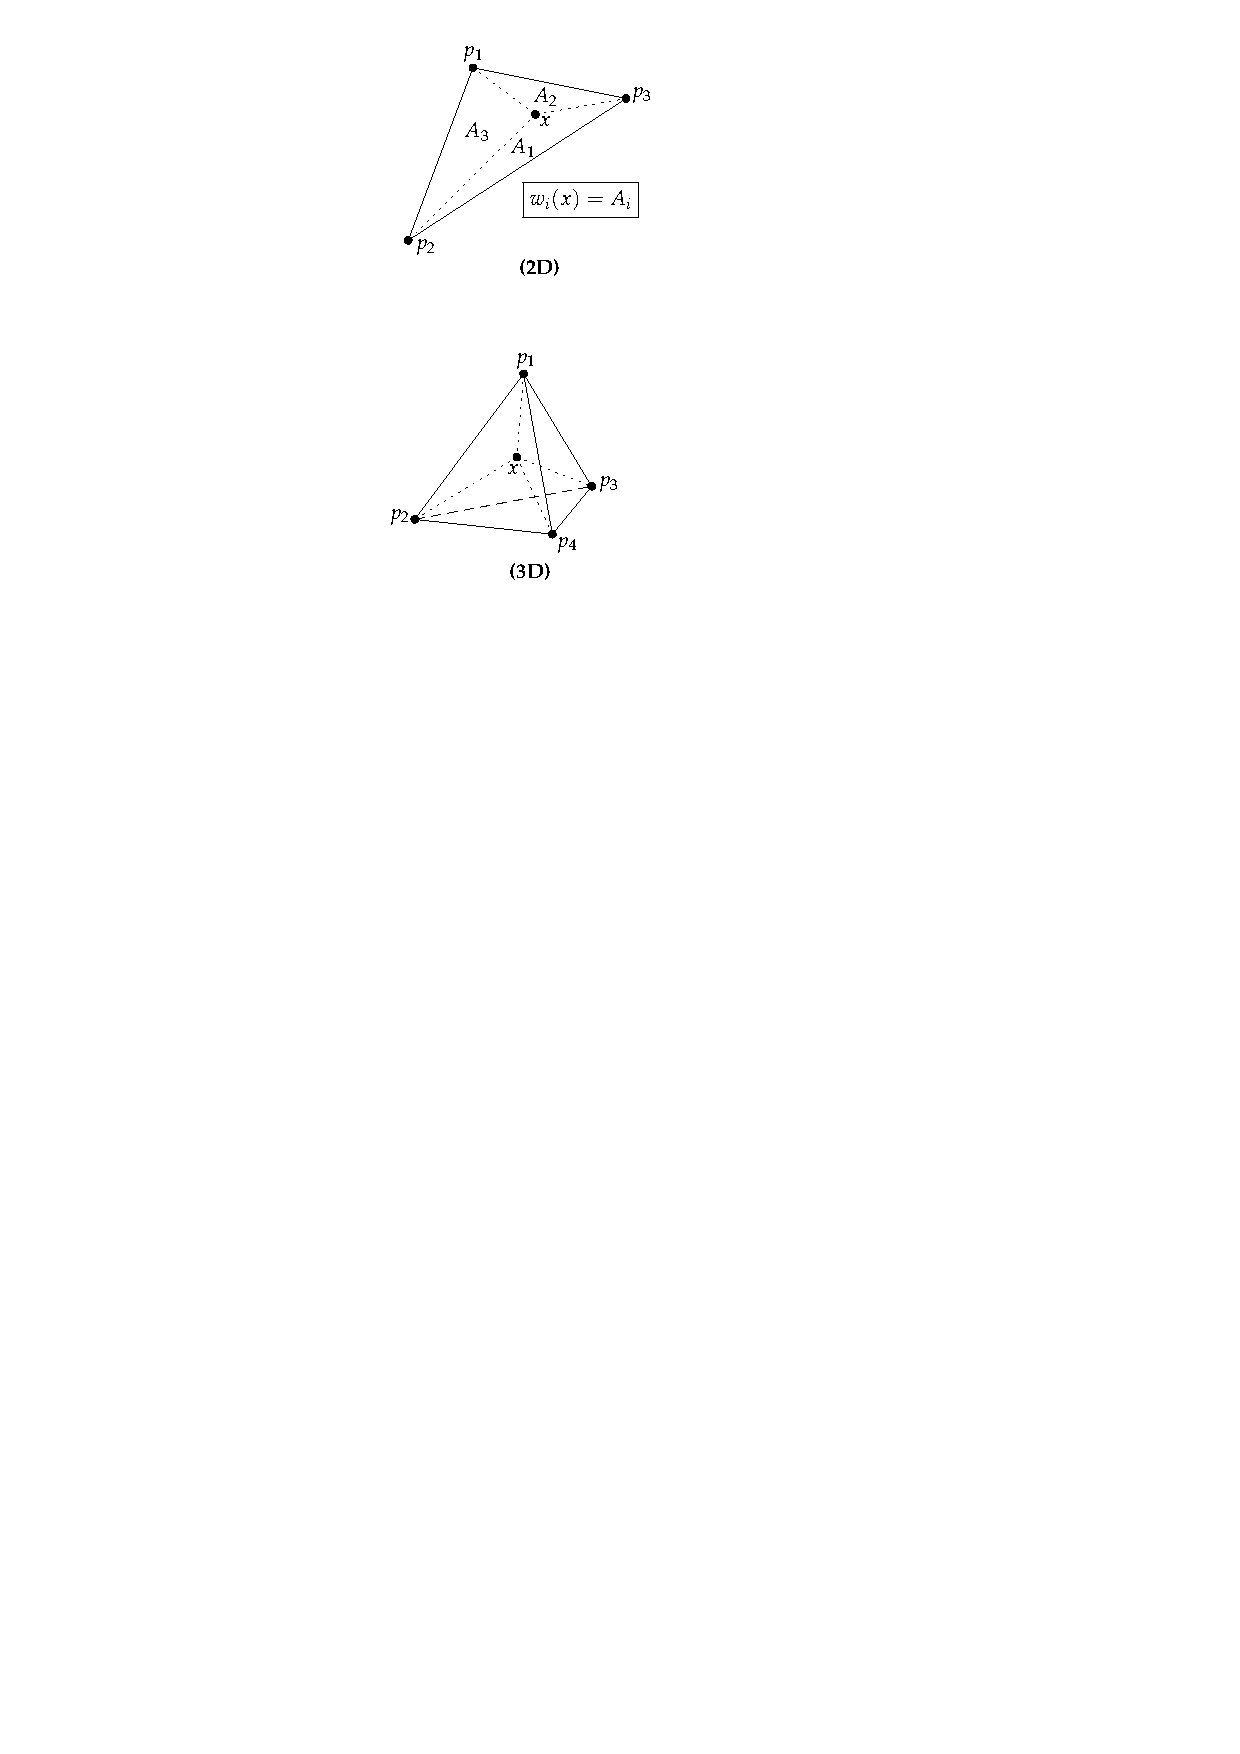
\includegraphics[width=0.9\textwidth]{figs/barycentric}
  \caption[Barycentric coordinates in two and three dimensions]{Barycentric coordinates in two and three dimensions. $A_i$ represents the area of the triangle formed by $x$ and one edge. In 3D, the tetrahedron is subdivided into 4 tetrahedra.}% 
\label{fig:barycentric}
\end{marginfigure}

The volume of a $d$-simplex $\sigma$ is easily computed:
\begin{equation}
vol(\sigma) = \frac{1}{d \, !} \left| \,  
                            \det \, \left( 
                                  \begin{array}{ccc}
                                    v^{0} & \cdots & v^{d} \\
                                    1     & \cdots & 1 \\
                                  \end{array}
                                \right)
                        \right|
\end{equation}  
where $v^{i}$ is a $d$-dimensional vector representing the coordinates of a vertex and $\det()$ is the determinant of the matrix. 

As explained above, finding tetrahedra having a good shape is not as easy as in two dimensions, and the presence of slivers yield bad results for the interpolation process. 
To be used in practice, the shape of the tetrahedra is usually improved with techniques involving the insertion of new points and/or applying flips.


%%%
\paragraph{Natural neighbour interpolation.}
The theory of this method also generalises in a straightforward manner to 3D.
Instead of having stolen areas, we have stolen \emph{volumes} between the Voronoi cells.
However, although the concepts behind the method are simple and easy to understand, its implementation for the 3D case is far from being straightforward. 
The main reasons are that it requires the computation of two VDs---one with and one without the interpolation point---and also the computation of volumes of Voronoi cells. 
This involves algorithms for both constructing a VD and deleting a point from it.

The volume of a $d$-dimensional Voronoi cell is computed by decomposing it into $d$-simplices---not necessarily Delaunay simplices---and summing their volumes. 
Triangulating a Voronoi cell is easily performed since it is a convex polyhedron.

%%%
\paragraph{kriging.}
All of the most common kriging varieties generalise to three dimensions without major changes, including simple kriging and ordinary kriging.
In the simplest case, covariance functions, experimental variograms and fitted functions work exactly the same as in 2D but are computed using distances in 3D.

However, the vertical direction has a much weaker correlation than the horizontal directions in many fields, \eg\ temperature, pressure and humidity.
Anisotropy is thus a much more significant factor in 3D and almost always has to be modelled.
A minimal solution is a custom distance function that scales the vertical direction.
A better (but still simple) solution involves computing multiple experimental variograms: two (for the horizontal plane \(x,y\) and for the vertical direction \(z\)) or three (for \(x\), \(y\) and \(z\)).

\subsection{Voxelised fields to points or surfaces}

The conversion of a voxel to a set of scattered points is not a simple operation.
Given a three-dimensional grid, it is possible to create one data point at the centre of each voxel.
Notice however that potentially a lot of the neighbouring points will be the same value, and thus a lot of redundancy is stored.

%

A better approach to this problem is to consider it as a simplification problem.%
\index{simplification}\marginnote{simplification}
Given a set $S$ of points in $\mathbb{R}^3$ representing a field $f$ (where each point $p$ in $S$ as an attribute $a$ attached to itself), the aim is to find a subset $R$ of $S$ which will approximate $f$ as accurately as possible, using as few points as possible. 
The subset $R$ will contain the `important' points of $S$, \ie\ a point $p$ is important when $a$ at location $p$ can not be accurately estimated by using the neighbours of $p$.

%

The two algorithms described in the GEO1015 book (Section~8.3) can in theory be generalised; Figure~\ref{fig:meshsimplification} shows the idea for the 1D case.
\begin{figure}
  \centering
  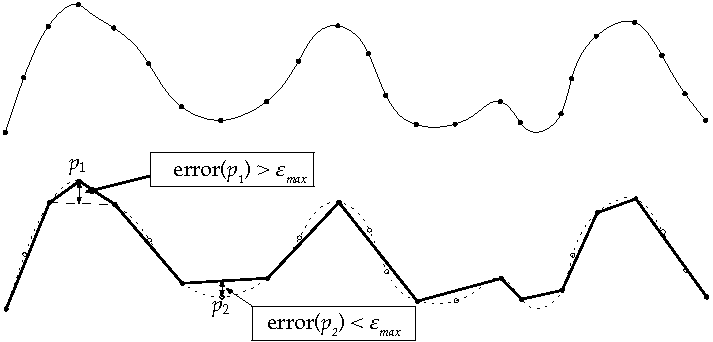
\includegraphics[width=0.85\linewidth]{figs/mesh_simplification}
  \caption[The importance measure of a point expressed by its error]{The importance measure of a point can be expressed by its error. When this error is greater than a given threshold $\epsilon_{\max}$, the point is kept ($p_1$), else it is discarded ($p_2$).}%
\label{fig:meshsimplification}
\end{figure}
Both strategies (decimation and refinement) can be implemented.

The error associated with each point $p$, denoted error($p$), is calculated by interpolating at location $p$ after $p$ has been temporarily removed from the field, and comparing the value obtained with the real attribute $a$ of $p$, thus error($p) = |a - estimation|$. 
As shown in Figure~\ref{fig:meshsimplification} for a one-dimensional case, when the error is more than $\epsilon_{\max}$ then the point must be kept, if it is less then the point can be discarded.

The method for 2D fields in GEO1015 uses linear interpolation in triangles, that is after $p$ has been temporarily deleted from DT($S$), the triangulation is updated and the estimation is obtained with the triangle containing location $p$. 
However, since mentioned earlier, using the DT in 3D for interpolation is not advised (because they contain slivers).
As an alternative, one could use for instance the natural neighbour interpolation, and each error is calculated by interpolating in the field at the location and comparing the real and the estimated value.

The principal and most known algorithm for extracting an isosurface form a voxel dataset is the \emph{Marching Cu\-bes}. 
The isosurface is computed by finding the intersections between the isosurface and each voxel/cube of the representation. 
Linear interpolation is used along the edges of each cube to extract `polygonal patches' of the isosurface. 
There exist 256 different cases for the intersection of a surface with a cube (considering that the value of each of the eight vertices of a cube is `above' of `under' the threshold), although if we consider the symmetry in a cube that comes down to only 15 cases. 
The major problem with the marching cubes algorithm is that the isosurface may contain `holes' or `cracks' when a cube is formed by certain configurations of above and under vertices. 
The ambiguities are shown in Figure~\ref{fig:isosurface_ambiguity} for the two-dimensional case when two vertices are above the threshold, and two under, and they form a `saddle'.
\begin{figure}
  \centering
  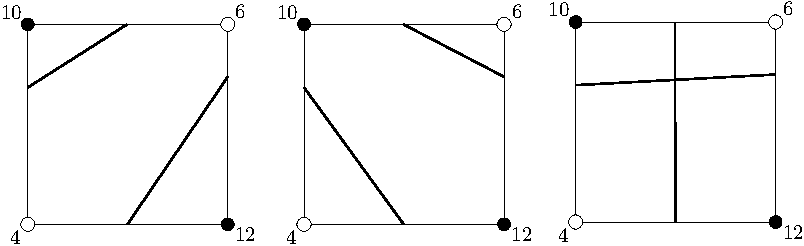
\includegraphics[width=0.7\textwidth]{figs/isosurface_ambiguity}
  \caption[Ambiguous extraction of an isoline]{Ambiguous extraction of an isoline where the attribute is 8.}% 
\label{fig:isosurface_ambiguity}
\end{figure}
The three-dimensional case is similar, with many more cases possible. 

\subsection{Voxelisation of objects}

In many cases, the data being voxelised consists of vector objects, either as a point cloud or a b-rep mesh.
We will thus explain a method to voxelise 0D, 1D, 2D and 3D vector objects.
In principle, it can be applied to arbitrary curves and surfaces, but in most instances they will be line segments (or polylines), as well as triangular and polygonal meshes.

\subsubsection*{Connectivity}

When rasterising a curve in 2D, different algorithms aim to obtain a pixellated curve that is connected according to either 4-connectivity or 8-connectivity (Figure~\ref{fig:rasterisation}).
These are as follows:
\begin{description}
\item[4-connectivity] means that pixels are connected to their four horizontally and vertically adjacent neighbours.
\item[8-connectivity] means that pixels are connected their four 4-connected neighbours and to their four diagonally incident neighbours.
\end{description}

\begin{figure}
\centering
\includegraphics[width=\linewidth]{figs/rasterisation}
\caption[Rasterising a line to achieve 4-connectivity and 8-connectivity]{Rasterising a line to achieve 4-connectivity (left) and 8-connectivity (right). The algorithm uses line targets (orange) that are intersected with the curve.}%
\label{fig:rasterisation}
\end{figure}

In 3D, the equivalent concepts are 6-connectivity, 18-connectivity and 26-connectivity.
These are as follows:
\begin{description}
\item[6-connectivity] \marginnote{6-connectivity}\index{6-connectivity} thus means that voxels are connected to their six adjacent neighbours (\ie\ on their left, right, front, back, bottom and top).
\item[18-connectivity] \marginnote{18-connectivity}\index{18-connectivity} means that voxels are connected to their six 6-connected neighbours and to their twelve incident neighbours that touch them diagonally along an edge (\ie\ top left, top right, top front, top back, bottom left, bottom right, bottom front, bottom back, front left, front right, back left and back right).
\item[26-connectivity] \marginnote{26-connectivity}\index{26-connectivity} means that voxels are connected to their eighteen 18-connected neighbours and to their eight incident neighbours that touch them diagonally along a vertex (\ie\ top front left, top front right, top back left, top back right, bottom front left, bottom front right, bottom back left and bottom back right).
\end{description}

An alternative way to think about these connectivities is that they are defined based on the dimensionality of the common boundary of the pixels or voxels.
6-connectivity means that two neighbouring voxels have a common 2D face.
18-connectivity means that they have at least a common 1D edge (which covers having a common 2D face).
26-connectivity means that they have at least a common 0D vertex (which covers having a common 1D edge or 2D face).

18-connectivity is an interesting concept that shows that there is a consistent logic for every dimension, but it is not really used in practice.
We will thus not discuss it further.

\subsubsection*{Intersections with targets (2D)}

In the example from Figure~\ref{fig:rasterisation}, the pixellated curve is obtained by calculating intersections between the original 1D curve and a set of \emph{intersection targets}\marginnote{intersection target}\index{intersection target} that are 1D line segments.
For 4-connectivity, the targets consist of the four line segments that bound every pixel.
For 8-connectivity, the targets are line segments that bisect the pixel horizontally and vertically and their midpoints.
The intersections with the targets give us a set of points, and the pixels in which these points are tell us the pixels that are part of the pixellated curve.
When a point lies on an edge between two pixels or a vertex between four pixels, we consider that all of the pixels are part of the curve.

In order to understand the logic of the targets, it is important to consider two aspects: (i) where the intersections will lie and (ii) whether they will detect lines when they do not cross the midpoint of a pixel.
For 4-connectivity, the targets simply detect when a line exits the pixel through the left, right, bottom or top edges on the \emph{boundary of the pixel}.
Since all intersections will be between pixels, the 2 or 4 pixels incident to the points will be part of the pixellated curve.
For 8-connectivity, the targets detect when they pass through the middle of the pixel either vertically or horizontally, which happens in the \emph{interior of the pixel}.
Crucially, note that they might do not detect when a line cuts through a corner of the pixel without crossing its middle vertically or horizontally.

Having covered the rasterisation of a 1D curve, let us discuss the two other cases: rasterising 0D points and 2D areas.
Since vector points are not connected, they do not need to be connected when rasterised either.
Since areas are always connected, they should also be connected when rasterised.
Connectivity is thus not an issue, which makes their rasterisation simpler.

An important observation for this method is that we used 1D targets to rasterise a 1D curve.
In order to rasterise a set of 0D points, we would use intersections with 2D targets, of which the optimal choice would consist of the whole area of each 2D pixel.
In order to rasterise a set of 2D areas, we would use intersections with 0D targets, of which the obvious choice is the midpoint of a pixel (although others are possible).
It is possible to see a duality property here: in order to rasterise \(i\)-dimensional objects, we use \((2-i)\)-dimensional targets.

\subsubsection*{Intersections with targets (3D)}

At this point, we should point out that the method described in the previous section is not the absolute fastest or the most common to rasterise objects in 2D.
However, it is a method with good performance with a logic that works perfectly in 3D, which is the reason why we will now explain how it works for voxelisation.

Let us start backwards, with the equivalent duality property for voxelisation, which states that we can use \((3-i)\)-dimensional targets to voxelise \(i\)-dimensional objects.
Using this formula directly, we can discuss the most obvious cases first: voxelising 0D points and 3D volumes, in which connectivity also does not matter.

In order to voxelise \textbf{0D points} (\eg\ a point cloud), we can thus simply use 3D targets that consist of the whole voxel (Figure~\ref{fig:points}).
That is, we can compute for each point which voxel it is in, or for each voxel the points that are in it.
This is a trivial operation using ranges of \(x\), \(y\) and \(z\) coordinates.

\begin{figure}
\centering
\begin{subfigure}[b]{\linewidth}
\includegraphics[width=\linewidth]{figs/points-pre}
\caption{}%
\label{subfig:points-pre}
\end{subfigure}
\\
\begin{subfigure}[b]{\linewidth}
\includegraphics[width=\linewidth]{figs/points-post}
\caption{}%
\label{subfig:points-post}
\end{subfigure}
\caption[A point cloud before and after voxelisation]{A point cloud (a) before and (b) after voxelisation. AHN data from Rotterdam.}%
\label{fig:points}
\end{figure}

Similar to the previous case, in order to voxelise \textbf{3D volumes}, we can use a 0D target with the midpoint of the voxel.
The exact form of this operation depends on the input data.
For instance, if we have tetrahedra as input, it would be a \emph{point in tetrahedron} operation, which could be done using barycentric coordinates.

Now, let us discuss the more challenging cases: 1D and 2D objects.
As with 1D curves in rasterisation, connectivity is important for these, so we will give targets that can be used in order to achieve 6-connectivity and 26-connectivity for each.

In order to voxelise \textbf{1D curves} with 6-connectivity (Figure~\ref{fig:lines}), we could detect when these pass through the top, bottom, left, right, front or back faces of the voxel using 2D targets (Figure~\ref{subfig:1d6}).
For 26-connectivity, we could detect when these pass through the middle of the voxel using three bisecting faces (Figure~\ref{subfig:1d26}).

\begin{figure}
\centering
\begin{subfigure}[b]{\linewidth}
\includegraphics[width=\linewidth]{figs/lines-pre}
\caption{}%
\label{subfig:lines-pre}
\end{subfigure}
\\
\begin{subfigure}[b]{\linewidth}
\includegraphics[width=\linewidth]{figs/lines-post}
\caption{}%
\label{subfig:lines-post}
\end{subfigure}
\caption[A set of lines before and after voxelisation]{A set of lines (a) before and (b) after voxelisation. OpenStreetMap data from Istanbul.}%
\label{fig:lines}
\end{figure}

\begin{figure}
\centering
\begin{subfigure}[b]{0.45\linewidth}
\includegraphics[width=\linewidth]{figs/1d6}
\caption{}%
\label{subfig:1d6}
\end{subfigure}
\quad
\begin{subfigure}[b]{0.45\linewidth}
\includegraphics[width=\linewidth]{figs/1d26}
\caption{}%
\label{subfig:1d26}
\end{subfigure}
\caption[Intersection targets for 1D curves for 6-connectivity and 26-connectivity]{Intersection targets (blue) for 1D curves for (a) 6-connectivity and (b) 26-connectivity.}%
\label{fig:1d}
\end{figure}

Now, in order to voxelise \textbf{2D surfaces} (Figure~\ref{fig:surfaces}) with 6-connectivity, we can use 1D targets that detect when we pass through any of the 12 edges on the boundary of the voxel (Figure~\ref{subfig:2d6}).
For 26-connectivity, we can use 1D targets that detect when we pass through the middle of the voxel (Figure~\ref{subfig:2d26}).

\begin{figure}
\centering
\includegraphics[width=\linewidth]{figs/surfaces}
\caption{Voxelising a surface}%
\label{fig:surfaces}
\end{figure}

\begin{figure}
\centering
\begin{subfigure}[b]{0.45\linewidth}
\includegraphics[width=\linewidth]{figs/2d6}
\caption{}%
\label{subfig:2d6}
\end{subfigure}
\quad
\begin{subfigure}[b]{0.45\linewidth}
\includegraphics[width=\linewidth]{figs/2d26}
\caption{}%
\label{subfig:2d26}
\end{subfigure}
\caption[Intersection targets for 2D surfaces for 6-connectivity and 26-connectivity]{Intersection targets (black lines) for 2D surfaces for (a) 6-connectivity and (b) 26-connectivity.}%
\label{fig:2d}
\end{figure}

%%%
%
\section{Exercises}

\begin{enumerate}
	\item Can you devise a formula to compare the space occupied by:
	\begin{enumerate}
		\item encoding all voxels in a grid linearly
		\item using a sparse encoding with individual voxels
		\item using an octree
	\end{enumerate}
	\item Can you think of cases where the rasterisation targets for 1D lines do not work? Hint: think of short curves.
	\item What kind of connectivity is used in the example of Figure~\ref{fig:lines}?
\end{enumerate}



%%%
%
\section{Notes and comments}

Voxels are widely used in areas other than geographic information.
For instance, both medical magnetic resonance (MRI) and computer tomography (CT) scans produce voxel models.
Physical simulations also use voxels since many calculations are easy to do using regular grid structures, \eg\ finite-element analysis.
Games sometimes use voxels as well, both for calculations and to render graphics.
It is worth noting that many of the techniques developed in these fields are just as applicable to geographic information as well.

4D grids using 3D+time are also sometimes used, both in geographic information and elsewhere.
Some of the earliest papers to mention this are: \citet{Mason94}, who implemented a system using a 4D grid of ocean temperatures with support for interpolation and generalisation operations, and \citet{Bernard98}, who implemented a 4D grid of atmospheric variables (\eg\ temperature, wind or pollution), which can be used for simulations.

\citet{Lorensen87} first describe the Marching Cubes algorithm to extract isosurfaces from voxels.
Although \citet{Wilhems90} describe various methods to fix the ambiguities, as is the case in two dimensions, the simplest solution is to subdivide the cubes into tetrahedra.

A common use of the representations covered here, especially voxel grids and octrees, is spatial indexing.
Cells can thus be used to store other kinds of data, \eg\ ids of objects, memory addresses with data, or a subset of a point cloud.

The original paper describing quadtrees is \citet{Finkel74}, whereas that for octrees is \citet{Meagher80}.
Bintrees~\citep{Samet85} are an alternative that split dimensions alternately rather than all at once.
If you are curious about more types of trees used in hierarhical subdivisions, have a look at the section titled `Spatial data partitioning trees' in this Wikipedia template: \url{https://en.wikipedia.org/wiki/Template:CS_trees}.

The voxelisation algorithm covered here is described by \citet{Laine13}, although it might be easier to understand the implementation described in \citet{Nourian16}.
Alternative targets to the ones described in this chapter are shown in both papers.
